
The startup times for each cluster deployment varied, being the most representative ones those obtained for the larger deployment: the 101-node cluster. In this case, the time needed by the rOCCI client to return all the resource endpoints corresponding to each VM ranged from 71 to 86 minutes. This is just the time to get the identifier corresponding to each VM instance, actually to have all the VMs running took longer: around 80 minutes more. So the total cluster startup time ranged from 2.5 to 3 hours. 

Some of the rOCCI requests failed with an \emph{execution expired} error and some of the VMs did not start. In the worst case 21 out of 101 failed.
%\begin{verbatim}
%An error occurred! Message: execution expired
%An error occurred! Message: HTTP Response status: [500] Internal Server Error!
%\end{verbatim}
We started to see this type of errors as soon as we tried to deploy, in a sequential way, more than 20 VMs at CESGA. In CESNET we could not do this analysis because there were only 10 VM slots available at the time of the benchmarks, due to a restriction in the amount of public IPs that they had available.

Trying to understand the source of this issue we tracked the performance of the OpenNebula frontend during the cluster startup. As it can be seen in Figure \ref{fig:on} the frontend experiences a high load several minutes after the start of the cluster deployment, this causes it to respond slower, probably producing the rOCCI execution expiration errors mentioned above. Looking at the processes in the OpenNebula frontend, we could see that this increase in the load is mainly due to the \emph{scp} processes launched to copy the image template to the OpenNebula nodes, more than 20 simultaneous scp processes seem to affect considerably the system performance, reducing its response times considerably.

% * Deploying 101 VMs:
%{{{
%[jlopez@test13 ~]$ time ./deploy_cluster_voms.sh &> deploy_cluster_voms.log
%
%real	71m31.677s
%user	1m43.104s
%sys	0m25.706s
%
%[jlopez@test13 ~]$ wc -l machines/pending
%98 machines/pending
%
%}}}
%

% Screenshot ganglia: 100 VMs deployment
\begin{figure}[t!]
\centering
%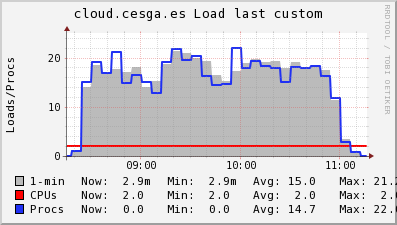
\includegraphics[width=0.74\textwidth]{figures/ON_load-complete.png}
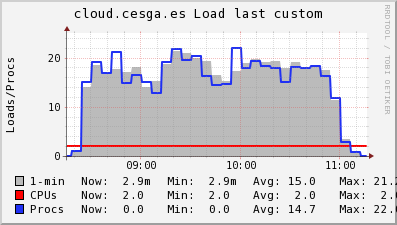
\includegraphics[width=0.6\textwidth]{figures/ON_load-complete.png}
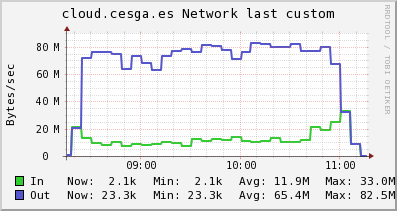
\includegraphics[width=0.6\textwidth]{figures/ON_network-complete.png}
\caption{OpenNebula frontend load and network usage graphs taken from Ganglia during the deployment of the 101 nodes cluster.}
\label{fig:on}
\end{figure}

%FedCloud does not count with a workload management system, so each VM creation request must be sent to the appropriate endpoint. This means that the partitioning of the cluster between the different FedCloud sites should be done in advance. In our case we run 10 VM at CESNET--the maximum possible at the time of the benchmarks--and the rest of them at CESGA--ranging from 10 to 91.

% Optimized startup times
In order to optimize the startup times we reduced the size of the image to 4GB and OpenNebula and OpenStack templates were re-configured to create on-the-fly an additional disk of 70GB, using a \emph{fs} disk type in OpenNebula and an \emph{ephemeral} disk in OpenStack. Additionally we modified the \emph{datastore} used in OpenNebula, so that the transfer manager (TM) used is \emph{shared} instead of \emph{ssh}. Since the instances are declared as non-persistent, this allows to perform a powerful optimization in the instance deployment process done by OpenNebula because the image copy process will be no longer done in a centralized way from the front-end node but in parallel from each node using a simple copy operation from the shared storage. The optimized startup times can be found in Table \ref{table:startupON}.

%% Table results startup OpenNebula
\begin{table}[h!]
\caption{Optimized startup times at CESGA after tuning OpenNebula configuration.}
\label{table:startupON}
%
\vspace{-0.5em}
%
\begin{center}
\begin{tabular}{ccl}
\toprule
Cluster size			& Startup time (s)	& Comments	  \\
\midrule
10                		& 249   		&	 \\
21                   		& 269			&        \\
51                   		& 822 			&        \\
101                  		& 1096			&        \\
%
\bottomrule
\multicolumn{3}{c}{\rule{0.98\textwidth}{0em}}\\
\rule{0.2\textwidth}{0cm} & \rule{0.2\textwidth}{0cm} &  \\
\end{tabular}
\end{center}
\end{table}



% Amazon EC2 startup times comparison
With the aim of comparing the startup times obtained with those of other commercial clouds we performed performed similar measurements of cluster startup times in Amazon EC2, this way we we can have a better understanding of how FedCloud performs compared to commercial clouds.

Amazon Elastic Compute Cloud (Amazon EC2) is a very popular commercial cloud platform that provides resizable compute capacity in a pay-per-use model. Even if the infrastructure behind Amazon EC2 is much larger than the one behind FedCloud, notice should be given to the fact that to launch more than 20 instances in Amazon EC2 you have to fill a form indicating the number of instances you need and their expected usage. For some users, especially commercial users, this requirement may be unnacceptable. This request is not validated automatically so you have to wait several hours until it is validated.
 
There are different tools available to create clusters in Amazon EC2, being Apache Whirr~\cite{whirr} one of the most popular. The Apache Whirr project started as a set of bash scripts distributed with Apache Hadoop for running Hadoop clusters on Amazon EC2, but it evolved to a Java version based on Apache jclouds~\cite{jclouds}, an open source multi-cloud toolkit that allows Whirr to support many different cloud providers. 
Unfortunately Whirr does not scale well due to the large number of REST requests it sends to the Amazon API that causes Amazon to temporarily block the client with a \emph{Request limit exceeded} error. The largest cluster we were able to launch in the eu-west-1 region was 21 nodes (see Table \ref{table:whirr}).

To avoid this issue we developed a custom tool~\cite{hadoopondemand} to create and configure the Hadoop cluster that used Amazon EC2 \emph{instance-count} functionality to request all the instances in the same REST request avoiding the \emph{Request limit exceeded} problem. The results are shown in Table \ref{table:ec2}. It can be seen that all the startup times are below 5 minutes. It should be taken into account that both the 51 and 101 cluster startups had all nodes that could not be reached for different reasons. In some cases the instance launch directly failed but in most cases the failing instances are just running correctly but they are not reachable from the other nodes in the cluster due to a security group internal network issue at Amazon.


%% Table results Amazon EC2: using whirr
\begin{table}[h!]
\caption{Amazon EC2 startup times using Whirr: the AMI and instance type used are also specified.}
\label{table:whirr}
%
\vspace{-0.5em}
%
\begin{center}
\begin{tabular}{cccc}
\toprule
Cluster size				& AMI				& Instance type		& Startup time (s) 	  \\
\midrule
10                   			& eu-west-1/ami-c37474b7 EBS	& t1.micro 		& 555   		  \\
10                   			& eu-west-1/ami-c37474b7 EBS	& m1.small		& 891			  \\
21                   			& eu-west-1/ami-c37474b7 EBS	& m1.small 		& 1670			  \\
31                   			& eu-west-1/ami-c37474b7 EBS	& m1.small 		& Fails  		  \\
%
\bottomrule
\multicolumn{4}{c}{\rule{0.98\textwidth}{0em}}\\
\rule{0.2\textwidth}{0cm} & \rule{0.4\textwidth}{0cm} & \rule{0.2\textwidth}{0cm} &  \rule{0.2\textwidth}{0cm} \\
\end{tabular}
\end{center}
%\vspace{-3.5em}
%\tablenotetext[a] {Identifies the configuration file where the parameter is set, the complete configuration files can be found at \url{https://github.com/grid-admin/hadoop}}
\end{table}

%% Table startup Amazon EC2: using our scripts
\begin{table}[h!]
\caption{Amazon EC2 startup times using our custom tool: the AMI used was \emph{eu-west-1/ami-54d43023} EBS plus instance store. The instance type used was \emph{m1.small} in all cases.}
\label{table:ec2}
%
\vspace{-0.5em}
%
\begin{center}
\begin{tabular}{ccl}
\toprule
Cluster size			& Startup time (s)	& Comments	  \\
\midrule
10                		& 191   		&	 \\
21                   		& 178			&        \\
51                   		& 583*			& 2 nodes not working       \\
101                  		& 276*			& 16 nodes not working       \\
101                  		& 297*			& 1 node not working       \\
%
\bottomrule
\multicolumn{3}{c}{\rule{0.98\textwidth}{0em}}\\
\rule{0.3\textwidth}{0cm} & \rule{0.3\textwidth}{0cm} &  \\
\end{tabular}
\end{center}
\end{table}

